% article_EN_5.0.tex — one-page presentation of WAC 5.0 for a DFIR magazine,
% English edition. The French edition is article_FR_5.0.tex, in this folder:
% both are maintained together, paragraph for paragraph. It follows the article
% on version 4.0 (article_EN_4.0.tex) and presents only what 5.0 adds.
%
% Build (LuaLaTeX, as the editor's recipe; build artefacts removed after):
%     ../build-docs.sh article/article_EN_5.0.tex
%
% Every figure comes from the validation and harmlessness files
% (doc/validation, doc/harmlessness) and the backlog, measured from 8 to
% 13 November 2026 on the code of 5.0. Backlog B-075.

\documentclass[10pt,a4paper,twocolumn]{article}
\usepackage[english]{babel}
\usepackage{fontspec}
\setmainfont{Noto Sans}
\setmonofont{DejaVu Sans Mono}[Scale=0.84]
\usepackage[top=13mm,bottom=13mm,left=14mm,right=14mm,columnsep=7mm]{geometry}
\usepackage{xcolor}
\usepackage{titlesec}
\usepackage{enumitem}
\usepackage{array}
\usepackage{graphicx}
\usepackage{caption}
\captionsetup{font={small,color=gris},skip=2pt}
\usepackage[hidelinks]{hyperref}
\definecolor{marine}{HTML}{0A1A33}
\definecolor{bleu}{HTML}{2F6DB5}
\definecolor{gris}{HTML}{5B6573}
\pagestyle{empty}
\setlength{\parindent}{0pt}
\setlength{\parskip}{0.35em}
\titleformat{\section}{\color{marine}\normalsize\bfseries}{}{0em}{}
\titlespacing*{\section}{0pt}{0.7em}{0.2em}
\setlist{nosep,leftmargin=1.1em}
\newcommand{\wac}{\textsc{wac}}
\newcommand{\fichier}[1]{\texttt{#1}}
\hypersetup{pdftitle={WAC 5.0 — applications' traces, dated right}}

\begin{document}

\twocolumn[{%
  {\color{marine}\LARGE\bfseries WAC 5.0: applications' traces, dated right}\par
  \vspace{0.3em}
  {\color{gris}Aerospace Cyber Defence Centre of Excellence (CEC), French Air and Space Force Academy}\par
  \vspace{0.6em}
  {\itshape \wac{} (Windows Artefacts Collector) is a free collector, in C++,
  that reads volumes raw and writes nothing on the examined machine, from XP~SP1
  to Windows~11 workstations and Server 2003 to 2025. Version 5.0 takes what
  applications keep outside the event logs, and dates each time written
  without a zone with the zone in force when it was written.}\par
  \vspace{0.9em}
}]

\section{97 products, one table}
Remote administration tools (TeamViewer, AnyDesk, RustDesk,
ScreenConnect\ldots), antivirus other than Defender, messaging, online storage,
file transfer, VPN, virtualisation, server applications and logs (Netlogon,
NPS, a certification authority), and what Windows keeps besides: 97 products in
eleven groups, each with its folders, most from KAPE's targets, and its switch
in \fichier{wac.yml}. PuTTY, WinSCP, WinRAR and 7-Zip are read in each user's
hive. The folders are read raw, like the rest: nothing is opened by the
system.

\section{Copied, then converted}
KAPE copies these files; \wac{} copies and converts them, without a decoder
per product: a log becomes one element per line, with the time it starts with;
XML, JSON and INI give their structure; a database or binary is listed and
stays in the exhibit store. A value named like a password, a private key block
of an OpenVPN profile, are never written: the JSON only says they exist. SSH
private keys are not taken; crash dumps and the Office cache, which may hold
documents, are off by default.

\section{The time written without a zone}
A clock time is not an instant. \wac{} converts it with the zone in force when
it was written, drawn from the System log: every change of offset since
Windows~10, the zone observed at boot and each day before. A change whose
instant no event gives stays an interval, never an invented instant; a time
lived twice gives its other possible instants. For each product present on the
test machines, the assumed zone was measured against the clock: a provoked
line, bracketed by the system time. TeamViewer, a line written under another
zone, October's repeated hour: dated to the millisecond, as Windows converts
them.

\section{What the review found}
The code and security review of 5.0 fixed two defects before release: a
private key of a text file would have come out in clear in the JSON, and a
forged NTFS index, naming a folder like its own pattern, looped the collection
into a stack overflow. Each has its test, seen failing before the fix; 5.0's
readers pass 46,000 mutated inputs with no read outside the buffer.

\section{What remains to be measured}
A witness proves that the table's path is taken, not that every version of a
product writes there: most of the 97 products were not installed on the test
machines, and their time is assumed local without verification. UltraViewer
writes its date in the format of the account's culture: it is not read. The
measured comparison with KAPE is still that of 29 October, before these
targets.

\section{In figures}
\begin{tabular}{@{}>{\raggedright\arraybackslash}p{0.75\columnwidth}@{\hspace{0.5em}}r@{}}
Artefacts collected (4.0: 87) & 99 \\
Products in the traces' table & 97 \\
Checks of the cycle, Windows~11 & 677 \\
Mutated inputs, 5.0's readers & 46,000 \\
Passwords or private keys written & 0 \\
\end{tabular}

\section{Availability}
Version 5.0.0, Windows~XP~SP1 to 11 and Server~2003 to 2025 (x86 and x64),
GPL~3.0 licence: \url{https://github.com/dev-cec/WAC}. Manuals, validation,
harmlessness and comparison files in French and English; cycles from 8 to
13 November 2026.

\vfill
\begin{center}
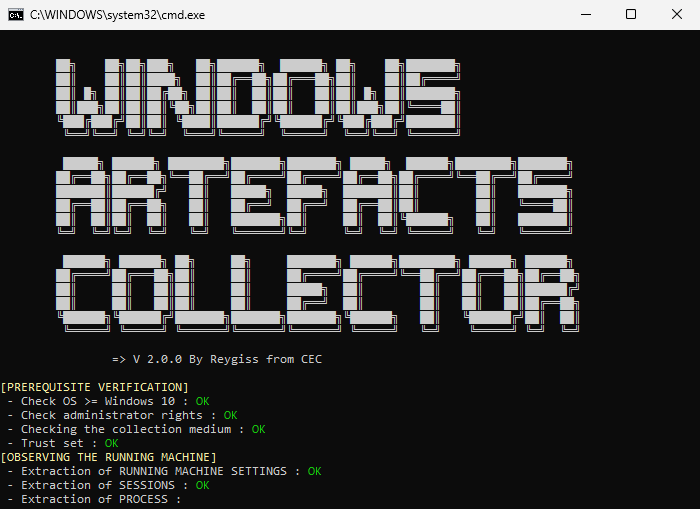
\includegraphics[width=\columnwidth,height=24mm,keepaspectratio]{../images/wac-running_EN.png}
\captionof*{figure}{\wac{} collecting.}
\end{center}

\end{document}
